\documentclass[12pt]{report}

\usepackage[margin=1in]{geometry}
\usepackage[math]{amznotes}
\usepackage[textsize=scriptsize]{todonotes}
\usepackage{xfrac}
\usepackage{enumitem}
\usepackage{tikz}
\usetikzlibrary{arrows,automata,positioning}

\title{\textbf{Algorithm Analysis and Automata}\\
\large UT Knoxville, Spring 2023, COSC 312}
\author{Dr. Michael W. Berry, Alex Zhang}

\begin{document}
\maketitle
\tableofcontents

\chapter{Introduction}
Computer science is all about problem-solving, and as computer scientists, we have developed a method of abstracting problems into three key components: unknowns, data, and conditions. To further our understanding of this process, we have developed the Theory of Computation (TOC), which encompasses three main areas: Automata, Computability, and Complexity.

Automata are problem-solving devices that help us model and solve problems. Computability provides a framework for categorizing these devices based on their computing power, while Complexity measures the space complexity of the tools we use to solve problems.

When approaching problems, we think of the data as ``words'' in a given ``alphabet'', while conditions form a set of words known as a language. The unknowns in this equation are boolean values, which are true if a word is in the language and false if it is not.

Overall, the Theory of Computation provides a framework for understanding how we solve problems using computers. By breaking down problems into their component parts, we can use automata to model and solve them, and categorize these solutions based on their computing power and space complexity.
\chapter{Finite Automata}

\begin{dfnbox}{Finite Automaton}{}
    A \dfntxt{finite automaton} is a theoretical device that is designed to recognize patterns in input from a set of characters. It operates through a finite set of states, including a start state and one or more final or accept states, and transitions between these states based on the input it receives.
\end{dfnbox}

In essence, a finite automaton is a simplified machine that helps to identify patterns within data. Finite automata can be used to generalize tons of applications, ranging from parsers for compilers, pattern recognition, speech processing, and market prediction.

\begin{exbox}{Simple Finite Automaton}{}
    \begin{center}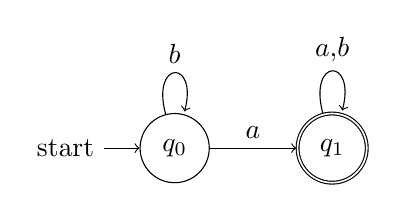
\begin{tikzpicture}[node distance=2cm, on grid, auto]
        \node[state, initial] (q0) {$q_0$};
        \node[state, accepting, right=of q0] (q1) {$q_1$};
        \path[->]
            (q0) edge node {$a$} (q1)
                 edge [loop above] node {$b$} ()
            (q1) edge [loop above] node {$a$,$b$} ();
    \end{tikzpicture}\end{center}
    Here, $q_0$ represents our start state, and $q_1$ represents our accept state. If we give the machine the character $a$, then it transitions to $q_1$ and is in an accept state. If we don't give it an $a$, then it will be stuck on $q_0$.
\end{exbox}

\begin{dfnbox}{Deterministic Finite Automaton (DFA)}{dfa}
    A \dfntxt{deterministic finite automaton} (DFA) is a type of finite automaton where every state transition corresponds to one and only one next state. In other words, a DFA is a finite-state machine that follows a single path of transitions for a given input.
    \tcblower
    We can formally define a DFA as a 5-tuple $(Q, \Sigma, \delta, q_0, F)$ where:
    \begin{itemize}[noitemsep]
        \item $Q$ is a finite set of all possible states
        \item $\Sigma$ is a finite set of symbols called an \dfntxt{alphabet}
        \item $\delta : Q \times \Sigma \to Q$ is a \dfntxt{transition function}
        \item $q_0 \in Q$ is the \dfntxt{start state}
        \item $F \subseteq Q$ is the set of \dfntxt{accept states} (or final states)
    \end{itemize}
\end{dfnbox}

The determinism of a DFA ensures that, for any given state and input, there is a unique and well-defined next state. To explain the computation of a DFA, let's consider a simple example DFA called $M_1$. The process of running $M_1$ can be broken down into the following steps:
\begin{itemize}[noitemsep]
    \item $M_1$ begins at its initial state.
    \item We give $M_1$ a sequence of characters from its alphabet.
    \item With each input symbol, $M_1$ makes a state transition along the edge labeled with that symbol.
    \item When $M_1$ reads the last symbol, it outputs whether it's in an accept state
\end{itemize}

In essence, the DFA computation involves moving from state to state based on the input symbols until the final state is reached, at which point it outputs whether the input is accepted or rejected.

\begin{dfnbox}{String}{}
    A \dfntxt{string} over an alphabet $\Sigma$ is a (finite) sequence of symbols in $\Sigma$.
    \begin{itemize}[noitemsep]
        \item $\epsilon$ represents the \dfntxt{empty string}
        \item The length of a string $w$ is denoted by $\abs{w}$.
        \item The \dfntxt{concatenation} of $w_1$ and $w_2$ is a string that contains one copy of $w_1$ followed by one copy of $w_2$. We simply denote this by juxtaposition: $w_1 w_2$.
    \end{itemize}
\end{dfnbox}

\begin{dfnbox}{Acceptance}{}
    We say a DFA \dfntxt{accepts} a string if, after reading that string, the machine ends on an accept state. Otherwise, the machine rejects the string.
    \tcblower
    More formally, let $M \coloneq (Q, \Sigma, \delta, q_0, F)$ be a DFA and $w = a_1 \ldots a_n$ be a string over $\Sigma$. We say $M$ \dfntxt{accepts} $w$ if there exists a sequence of states $r_0 \ldots r_n$ in $Q$ such that:
    \begin{itemize}[noitemsep]
        \item $r_0 = q_0$
        \item $\delta(r_i, a_{i+1}) = r_{i+1}$
        \item $r_n \in F$
    \end{itemize}
\end{dfnbox}

\begin{dfnbox}{Language}{}
    A \dfntxt{language} is simply a set of strings. A language over an alphabet means every character of every string in the language is a character of the alphabet.
\end{dfnbox}

\begin{tecbox}{Constructing a DFA}{}
    Here's the general design approach for a DFA:
    \begin{enumerate}[noitemsep]
        \item Identify the possible states of the finite automaton
        \item Identify the condition to change from one state to another
        \item Identify initial and final states
        \item Add missing transitions
    \end{enumerate}
\end{tecbox}

Given a finite automaton, we can deduce the language of possible inputs.

\begin{exbox}{Simple Finite Automaton}{}
    Let $M_1 \coloneq (Q, \Sigma, \delta, q_1, F)$ where $Q = \{q_1, q_2, q_3\}$, $\Sigma = \{0, 1\}$, and $F = \{q_2\}$. Define a possible transition function $\delta$.
    \tcblower
    The transition function $\delta : Q \times \Sigma \to Q$ must map every ordered pair of a state and letter to another state.

    \begin{center}\begin{tabular}{c | c | c }
        & 0 & 1 \\ \hline
        $q_1$ & $q_1$ & $q_2$ \\
        $q_2$ & $q_3$ & $q_2$ \\
        $q_3$ & $q_2$ & $q_2$
    \end{tabular}\end{center}

    Then, the language is:
    \[ L(M_1) = \left\{ (w \in \Sigma^*: 1 \in w) \land (\text{has even number of 0s following the last 1}) \right\} \]
\end{exbox}

\begin{exbox}{Simple Finite Automaton}{}
    Let $M_2 \coloneq (Q, \Sigma, \delta, q_1, F)$ where $Q = \{q_1, q_2\}$, $\Sigma = \{0, 1\}$, and $F = \{q_2\}$. Consider a possible transition function $\delta$ defined as such:

    \begin{center}\begin{tabular}{c | c | c }
        & 0 & 1 \\ \hline
        $q_1$ & $q_1$ & $q_2$ \\
        $q_2$ & $q_1$ & $q_2$ \\
    \end{tabular}\end{center}

    This time, our language is much simpler:
    \[ L(M_2) = \{ w \in \Sigma^* : w\ \text{ends in a 1} \} \]

    Now imagine if kept everything the same but made $F = \{q_1\}$. Because our finite automaton's initial state is $q_1$, we must now consider the possibility of the empty word. Then our language is:
    \[ L(M_2) = \{ w \in \Sigma^* : w\ \text{ does not end in 1} \} \]
\end{exbox}

\begin{exbox}{Pattern Recognizing Finite Automaton}{}
    Let $M_3 \coloneq (Q, \Sigma, \delta, q_1, F)$ where $Q = \{s, q_1, q_2, r_1, r_2\}$, $\Sigma = \{a, b\}$, and $F = \{q_1, r_1\}$. Consider a possible transition function $\delta$ defined as such:

    \begin{center}\begin{tabular}{c | c | c }
        & 0 & 1 \\ \hline
        $s$ & $q_1$ & $r_1$ \\
        $q_1$ & $q_1$ & $q_2$ \\
        $q_2$ & $q_1$ & $q_2$ \\
        $r_1$ & $r_2$ & $r_1$ \\
        $r_2$ & $r_2$ & $r_1$ \\
    \end{tabular}\end{center}

    Now our machine encompasses two smaller machines. $s$ acts as a branch point where we must lock ourselves into either $q$ states or $r$ states.

    % \begin{center}\begin{tikzpicture}
    %     \begin{scope}[every node/.style={circle,thick,draw}]
    %         \node (s) at (0,0) {s};
    %         \node (q1) at (-2,-3) {q1};
    %         \node (q2) at (-2, -6) {q2};
    %         \node (r1) at (2,-3) {r1};
    %         \node (r2) at (2, -6) {r2};
    %     \end{scope}

    %     \begin{scope}[>={Stealth[black]},
    %           every node/.style={fill=white,circle},
    %           every edge/.style={draw=red,very thick}]
    %         \path [->] (s) edge node {$a$} (q1);
    %         \path [->] (s) edge node {$b$} (r1);
    %         \path [->] (q1) edge node {$b$} (q2);
    %         \path [->] (r1) edge node {$a$} (r2);
    %     \end{scope}
    % \end{tikzpicture}\end{center}

    Then our language is:
    \[ L(M_3) = \{ w \in \Sigma^* : (w\ \text{starts and ends with}\ a) \lor (w\ \text{starts and ends with}\ b) \} \]
\end{exbox}

Now, let's start with a given language, then find an acceptable transition function $\delta$.
\begin{exbox}{Finding $\delta$ from Language}{}
    Suppose $\Sigma = \{a, b\}$. Let $F_1$ be a finite automaton that recognizes the language $A_1 \coloneq \{w : w\ \text{has at exactly two a's} \}$. Let $F_2$ be a finite automaton that recognizes the language $A_2 \coloneq \{w : w\ \text{has at least two b's} \}$.

    % \begin{center}\begin{tikzpicture}
    %     \begin{scope}[every node/.style={circle,thick,draw}]
    %         \node (1) at (0,0) {};
    %         \node (2) at (3,0) {};
    %         \node (3) at (6,0) {};
    %         \node (4) at (9,0) {};
    %     \end{scope}

    %     \begin{scope}[>={Stealth[black]},
    %           every node/.style={fill=white,circle},
    %           every edge/.style={draw=red,very thick}]
    %         \path [->] (1) edge [loop above] node {$b$} (1);
    %         \path [->] (1) edge node {$a$} (2);
    %         \path [->] (2) edge [loop above] node {$b$} (2);
    %         \path [->] (2) edge node {$a$} (3);
    %         \path [->] (3) edge [loop above] node {$b$} (3);
    %         \path [->] (3) edge node {$a$} (4);
    %         \path [->] (4) edge [loop above] node {$a,b$} (4);
    %     \end{scope}
    % \end{tikzpicture}\end{center}
\end{exbox}
\todo{Finish example}


\chapter{Regular Languages}

\begin{dfnbox}{Regular Language}{}
    A language is \dfntxt{regular} if there exists a finite automaton that can accept every string from the language.
\end{dfnbox}

We can consider new languages derived from set operations on other languages, such as union and concatenation. There are also two special operations to consider: \dfntxt{concatenation} and \dfntxt{Kleene closure}.

\begin{dfnbox}{Concatenation}{}
    Let $L_1$ and $L_2$ be languages. The \dfntxt{concatenation} of $L_1$ and $L_2$ is defined as:
    \[ L_1 \circ L_2 \coloneq \{ xy : x \in L_1 \land y \in L_2 \} \]
\end{dfnbox}

\begin{dfnbox}{Set Power, Kleene Closure}{}
    Let $L$ be a language, and let $n \in \N$. The \dfntxt{set power} operation on $L$ is defined as:
    \begin{align*}
        L^n &\coloneq \begin{cases}
            \{\epsilon\}, & \text{if}\ n = 0  \\
            L^{n-1} \circ L, & \text{otherwise}
        \end{cases} \\
        &= \underbrace{L \circ L \circ \cdots \circ L}_{n\ \text{times}}
    \end{align*}
    The \dfntxt{Kleene closure} of $L$ is defined as:
    \begin{align*}
        L^* &\coloneq \bigcup_{i = 0}^\infty L^i \\
        &= L^0 \circ L^1 \circ L^2 \circ \cdots
    \end{align*}
    %\[ A^* \coloneq \{ x_1 \ldots x_k : k \geq 0, x_i \in A, 0 \leq i \leq k \} \]
\end{dfnbox}

\begin{thmbox}{Closure of Regular Languages}{}
    Class of regular languages is closed under intersection and closed under complementation.
\end{thmbox}
\todo{Need proof here!}

\section{Nondeterminism}

Designing a DFA that accepts a complex language can be a challenging task. However, to address this, we can introduce the concept of nondeterminism, which allows the machine to choose state transitions even without any input. By doing so, we create a more flexible automaton that can branch and handle complex languages. Specifically, we can create a nondeterministic finite automaton (NFA) that can recognize languages beyond the capability of a DFA.

% \begin{dfnbox}{Nondeterministic Computation}{}
%     A machine that is \dfntxt{nondeterministic} is allowed to choose its next state.
% \end{dfnbox}

\begin{dfnbox}{Nondeterministic Finite Automaton (NFA)}{}
    A \dfntxt{nondeterministic finite automaton} is a finite automaton where each state transition can lead to an arbitrary number of states, chosen by the machine.
    \tcblower
    We can formally define an NFA as a 5-tuple $(Q, \Sigma, \delta, q_0, F)$ where:
    \begin{itemize}[noitemsep]
        \item $Q$ is a finite set of states
        \item $\Sigma$ is a finite set of symbols called an \dfntxt{alphabet}
        \item $\delta : Q \times (\Sigma \cup \{ \epsilon\}) \to \mathcal{P}(Q)$ is a \dfntxt{transition function} ($\mathcal{P}(Q)$ being the powerset of $Q$)
        \item $q_0 \in Q$ is the \dfntxt{start state}
        \item $F \subseteq Q$ is the set of \dfntxt{accept states}
    \end{itemize}
    In this context, $\epsilon$ represents a nondeterministic choice by the machine.
\end{dfnbox}

With a nondeterministic finite automaton (NFA), a state can have multiple transitions for a given input symbol, creating multiple paths the machine can follow. This makes it easier to design an NFA that accepts a more complex language, as the machine can explore different paths to find the correct one. However, this flexibility comes at a cost: NFAs are more difficult to analyze and simulate compared to DFAs.

\begin{dfnbox}{Acceptance (NFA)}{}
    An NFA \dfntxt{accepts} a string if, after reading that string, the NFA ends on an accept state.
    \tcblower
    More formally, let $N \coloneq (Q, \Sigma, \delta, q_0, F)$ be an NFA and $w \coloneq y_1 \ldots y_n$ be a string over $\Sigma \cup \{\epsilon\}$. We say $N$ \dfntxt{accepts} $w$ if there exists a sequence of states $r_0, \ldots, r_m \in Q$ such that:
    \begin{enumerate}[noitemsep]
        \item $r_0 = q_0$
        \item $\delta(r_i, y_{i+1}) = r_{i+1}$ for $i = 0, \ldots, m-1$
        \item $r_m \in F$.
    \end{enumerate}
\end{dfnbox}

\begin{thmbox}{Closure of Regular Languages}{}
    The class of regular languages is closed under the union operation.
    \tcblower
    \begin{proof}[Proof sketch]
    \end{proof}
\end{thmbox}
\todo{draw proof sketch here}


\section{DFA/NFA Equivalence}

An NFA can have multiple state transitions for a given input symbol, leading to ambiguity in the possible paths the machine can take. To overcome this ambiguity, we can ``blow up'' the set of possible states to its power set. This means creating a new state for every possible combination of states the NFA could be in at any given time.

Once we have this expanded set of states, we can create deterministic transitions between the subsets of states. This means that for every input symbol, there is only one possible state the machine can transition to. By doing this, we shift the ambiguity from the transitions between states to the states themselves. The result is a DFA that is more predictable and easier to analyze.

\begin{tecbox}{Converting NFA to DFA}{}
    To convert an NFA to a DFA, we carry out the following steps:
    \begin{enumerate}
        \item Let $N \coloneq (Q, \Sigma, \delta, q_0, F)$ be an NFA that recognizes the language $A$.
        \item Construct the DFA $M$ that also recognizes $A$. For convenience, define:
        \[ M \coloneq (Q\prime, \Sigma, \delta\prime, q_0\prime, F\prime) \]
        \item For all $R \subseteq Q$, define $E(R)$ to be the collection of all states that can be reached from $R$ by going along $\epsilon$ transitions, including members of $R$ themselves.
        \item Modify $\delta\prime$ to place additional edges on all states that can be reached by going along $\epsilon$ edges after every step.
        \item Set $q_0\prime = E(\{q_0\})$ and $F\prime = \{ R \in Q\prime : R\ \text{contains an accept state of}\ N \}$.
    \end{enumerate}
\end{tecbox}

\todo{examples of NFA/DFA equivalence here}

\chapter{Irregular Languages}
\begin{dfnbox}{Regular Expression (RE)}{}
    We say that $R$ is a \dfntxt{Regular expression} if $R$ is one of the following:
    \begin{itemize}[noitemsep]
        \item $a$ for some $a \in \Sigma$ (a symbol of the alphabet)
        \item $\epsilon$ (language contains only the empty string)
        \item $\emptyset$ (language contains no strings)
        \item $(R_1 \cup R_2)$, where $R_1$ and $R_2$ are regular expressions
        \item $(R_1 \circ R_2)$, where $R_1$ and $R_2$ are regular expressions
        \item $R_1^*$, where $R_1$ is a regular expression
    \end{itemize}
\end{dfnbox}
\todo{what the hell is this definition}

\begin{thmbox}{}{}
    A language is regular if and only if some regular expression describes it.
    \tcblower
    \begin{proof}
        If a language $R$ is described by a regular expression, then $A$ is recognized by an NFA. Thus, $A$ must be regular. If the language $R$ is regular, then it is recognized by a DFA from which a regular expression can be deduced.
    \end{proof}
\end{thmbox}

\begin{exbox}{Irregular Languages}{}
    Consider the following languages:
    \begin{itemize}[noitemsep]
        \item $B = \{ 0^n 1^n : n \geq 0\}$ is not regular.
        \item $C = \{ w : w\ \text{has an equal number of 0s and 1s} \}$ is not regular. We would need infinite states to account for all possible inputs.
        \item $D = \{ w : w\ \text{has an equal number of 01 and 10 substrings} \}$ is regular. We can think of this as recording transitions between 0s and 1s, and vice versa. In this sense, every 01 must be eventually followed by a 10, and every 10 must be eventually followed by a 01.
    \end{itemize}
\end{exbox}

\section{Pumping Lemma}
The pumping lemma is a powerful tool in the theory of computation that helps us reason about the limitations of regular languages. Regular languages are those that can be recognized by a finite automaton, but not all languages are regular. The pumping lemma provides a way to prove that certain languages are not regular by demonstrating that they cannot satisfy certain conditions.

The pumping lemma works by breaking a long string in a language into smaller parts in a way that exposes its structure. If the language is regular, then we should be able to divide the string into parts in such a way that each part can be repeated or removed to create a new string that is still in the language. However, if the language is not regular, then at some point we will reach a part that cannot be repeated or removed without breaking the rules of the language.

% \begin{dfnbox}{Pumping, Pumping Length}{}
%     All strings in a language can be \dfntxt{pumped} if they are as long or longer than a specified \dfntxt{pumping length}.
% \end{dfnbox}

% In other words, every string contains a section that can be repeated any number of times, and the resulting string is still in the language. For example, we can write sqrt(sqrt(sqrt($\ldots$(sqrt($x$))$\ldots$))) in C, and it's still valid.

\begin{thmbox}{Pumping Lemma}{pl}
    Let $L$ be a regular language. There exists a pumping length $p \in \N$ such that, for any string $s$ of length $p$ or more, $s$ may be divided into three substrings, $s = x y z$ where all the following hold:
    \begin{enumerate}[noitemsep]
        \item $\forall (n \geq 0) \left( x y^n z \in L \right)$
        \item $\abs{y} > 0$
        \item $\abs{x y} \leq p$
    \end{enumerate}
    \tcblower
    \begin{proof}[Proof sketch]
        As a guide, the proof follows this general form:
        \begin{itemize}[noitemsep]
            \item Let $M \coloneq (Q, \Sigma, \delta, q_1, F)$ be a DFA that recognizes $A$. Let $p$ be the number of states.
            \item Show that any string $s \in A$ where $\abs{s} \geq p$ can be broken into $xyz$ satisfying the three conditions.
            \item If there are no strings in $A$ of length $p$ or more, then the lemma is true because all three conditions hold for all strings of length $p$ or more.
        \end{itemize}
    \end{proof}

    A formal proof is as follows:
    \begin{proof}
        Let $M \coloneq  (Q, \Sigma, \delta, q_1, F)$ be a DFA that recognizes $A$. Let $p \coloneq \abs{Q}$. Let $s \coloneq s_1 s_2 \ldots s_n$ be a string over $\Sigma$ with $n \geq p$ and $r = r_1 r_2 \ldots r_{n+1}$ be the sequence of states encountered while processing $s$.\todo[inline]{TODO: finish proof}
    \end{proof}
\end{thmbox}

\begin{tecbox}{Proving a Language is Irregular}{}
    To prove that a language $A$ is not regular, we:
    \begin{enumerate}
        \item Suppose for contradiction $A$ is regular
        \item Find $s \in A$ where $\abs{s} \geq p$ that cannot be pumped; consider all the ways of dividing $s$ into $xyz$, and show that for each division, at least one of the conditions fail.
    \end{enumerate}
\end{tecbox}

\begin{exbox}{Simple Pumping Lemma Example}{}
    Prove that the language $B \coloneq \{ 0^n 1^n : n \geq 0 \}$ is not regular.
    \tcblower
    We can show that any substring of $B$ cannot be pumped by contradicting the first condition of the \nameref{thm:pl}.
    \begin{proof}
        Suppose for contradiction $B$ is regular. Let $p$ be the pumping length for $B$. Let $s \coloneq 0^p1^p \in B$. Then $\abs{s} = 2p > p$. By the \nameref{thm:pl}, we can partition $s$ into three substrings, say $x,y,z$, such that $x  y^*  z \in B$. Let $s\prime \coloneq x  y  y  z$. WE will show $s\prime \notin B$. Consider the three possible cases for the contents of $y$:
        \begin{enumerate}
            \item $y \in 0^+$. Then. $s\prime$ has more $0$s than $1$s. Thus, $s\prime \notin B$, contradicting the first condition of the \nameref{thm:pl}.
            \item $y \in 1^+$. Then, following the logic from the first case, this is not possible.
            \item $y$ consists of $0$s and $1$s. Then $y  y \notin 0^n1^n$, so $s \prime \notin B$.
        \end{enumerate}
    \end{proof}

    We can simplify the above proof by targeting condition 3 instead:
    \begin{proof}
        By the third condition of the \nameref{thm:pl}, we have $\abs{x  y} \leq p$. Hence, $y$ could only contain $0$s.
    \end{proof}
\end{exbox}

\begin{exbox}{Another Pumping Lemma Example}{}
    Prove that the language $E \coloneq \left\{ 0^i 1^j : i > j \right\}$ is not regular.
    \tcblower
    \begin{proof}
        Suppose for contradiction $E$ is regular. Let $p$ be the pumping length for $E$, and let $s \coloneq 0^{p+1}1^p \in E$. Then $\abs{s} = (p+1) + p > p$. By the \nameref{thm:pl}, we can partition $s$ into three substrings, say $x,y,z$, such that $x  y^*  z \in E$. Then, by the third condition, we have $\abs{x  y} \leq p$. Note that there are $p+1$ number of $0$s at the beginning of $s$. Thus, $x \in 0^*$ and $y \in 0^+$. Consider the case when $i = 0$. Then $x  y^+  z \notin E$, leaving only $x  z$. However, $\abs{y} > 0$ by the second condition, so $x  z$ would lose at least one $0$. Thus, $x  z \notin E$, so $x  y^*  z \notin E$. Therefore, $E$ is not regular.
    \end{proof}
\end{exbox}

\chapter{Context-Free Languages}
Certain languages like $L \coloneq \{ 0^n 1^n : n \geq 0 \}$ cannot be specified by neither a finite automaton nor a regular expression. To address this, we can use context-free grammars to specify a much larger class of languages.

\begin{dfnbox}{Context-Free Grammar (CFG)}{}
    A context-free grammar consists of a set of production rules that describe how to generate strings. The rules consist of a left-hand side symbol and a right-hand side string.
    \tcblower
    More formally, a \dfntxt{context-free grammar} can be defined as 4-tuple $(V, \Sigma, R, S)$ where:
    \begin{itemize}[noitemsep]
        \item $V$ is a finite set of symbols called \dfntxt{variables} or \dfntxt{non-terminals}
        \item $\Sigma$ is a finite set of symbols disjoint from $V$ called \dfntxt{terminals}
        \item $R$ is a finite relation from $V$ to $(V \cup \Sigma)^*$ (i.e. a set of \dfntxt{production rules})
        \item $S \in V$ is the \dfntxt{start variable}
    \end{itemize}
    Instead of writing $(a, b) \in R$, we write $a \to b$.
\end{dfnbox}

To generate a string using a CFG, we begin with the start variable $S$. Then, we repeatedly apply the production rules in $R$ to replace a variable with a sequence of symbols until no variables remain in the string. In each step, we choose a variable in the string and use a production rule that has that variable on the left-hand side to generate a new sequence of symbols to replace that variable on the right-hand side. We repeat this process until we have a string consisting only of terminal symbols from $T$.

% A CFG generates strings by the following steps:
% \begin{enumerate}[noitemsep]
%     \item Begin with the start variable $S \in V$.
%     \item Use a rule in $R$ to convert a symbol of the string to another symbol.
%     \item Repeat 2 and 3 until no variables remain in the string.
% \end{enumerate}

\begin{exbox}{Simple CFG}{}
    Suppose CFG $G_1$ has the following specification rules:
    \begin{align*}
        A &\mapsto 0A1 \\
        A &\mapsto B \\
        B &\mapsto \#
    \end{align*}
    The start variable for $G_1$ is $A$. The non-terminals are $A$ and $B$. The terminals are $0$, $1$, and $\#$. An example output may look like:
    \[ 0A1, 00A11, 000A111, 0000B111, 000\#111 \]
    We can add a rule like $B \mapsto \epsilon$ to erase strings. Then the final output would be $000111$.
    \tcblower
    \textbf{Derivation:}
    \[ A \to 0A1 \to 00A11 \to 000A1111 \to 000B111 \to 000\#111 \]
\end{exbox}

\begin{dfnbox}{Direct Derivation}{}
    If $uv,w, \in (V \cup \Epsilon)^*$ and $A \mapsto w \in R$ is a grammar rule, then we say that $uvw$ is \dfntxt{directly derived} from $uAv$ using the rule $A \to w$.
\end{dfnbox}

\begin{exbox}{Language of Simple CFG}{}
    Let $G_3 \coloneq (\{S\}, \{a,b\}, \{S \to aSb | SS | \epsilon\}, S)$ be a CFG. $L(G_3)$ is the language of all strings of properly-nested pair-delimiters (e.g. parentheses or brackets).
\end{exbox}

\begin{exbox}{Another Language of Simple CFG}{}
    Let $G_3 \coloneq (\{E,T,F\}, \{a, +, *, (, )\}, R, E)$ where $R$ is given by:
    \[ E \mapsto E + T | T,\quad T \mapsto T * F | F,\quad F \mapsto (E) | a \]
    $L(G_4)$ is the language of some arithmetic expressions.
\end{exbox}

\begin{dfnbox}{Ambiguous Grammar}{}
    A grammar is considered \dfntxt{ambiguous} if it can generate the same string in different ways.
\end{dfnbox}

\section{Design Techniques}
Many CFGs are unions of simpler CFGs. Combination involves putting all the rules together and adding the new rules.



\amzindex
\end{document}
